\documentclass[tikz,border=2mm]{standalone}
\usetikzlibrary{calc,quotes,intersections, angles}

\begin{document}
    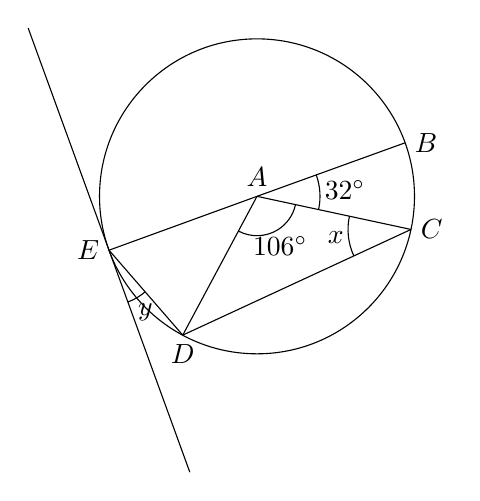
\begin{tikzpicture}[scale=2]
    % mark points on circle
        \coordinate[label=above:$A$] (A) at (0,0);
        \coordinate[label=left:$E$] (E) at (-160:1);

    % draw chords and circle
        \draw[name path=circ] (0,0) circle (1);
        \draw (E) -- (A);
        
    % draw tangent
    \draw (E) -- ($(E)!1.5!-90:(A)$) coordinate (L);
    \draw (E) -- ($(E)!1.5!90:(A)$) coordinate (M);

    % % %
    \path[name path=ED] (E) -- ($(E)!1!21:(L)$);
    \path[name intersections={of=ED and circ, by={temp,D}}];
    \path[name path=AC] (A) -- ($(A)!1.1!106:(D)$);
    \path[name intersections={of=AC and circ, by={C,temp}}];
    \path[name path=AB] (A) -- ($(A)!1.1!32:(C)$);
    \path[name intersections={of=AB and circ, by={B,temp}}];

    \draw (E) -- (D);
    \draw (A) -- (D);
    \draw (A) -- (C);
    \draw (A) -- (B);
    % % Label points C and B
    \node at (D) [anchor=north] {$D$};
    \node at (C) [anchor= west] {$C$};
    \node at (B) [anchor = west] {$B$};

    \draw (C) -- (D);
    
    \pic [draw, "$y$", angle eccentricity=1.3, angle radius = 0.7cm] {angle = L--E--D};
    \pic [draw, "$x$", angle eccentricity=1.2, angle radius = 0.8cm] {angle = A--C--D};
    \pic [draw, "$32^\circ$", angle eccentricity=1.4, angle radius = 0.8cm] {angle = C--A--B};
    \pic [draw, "$106^\circ$", angle eccentricity=1.4, angle radius = 0.5cm] {angle = D--A--C};
        
    \end{tikzpicture}
\end{document}